\documentclass{article}

% pacakages
\usepackage{amsmath, amsfonts, amssymb}
\usepackage{stmaryrd}
\usepackage{fancyhdr}
\usepackage{lastpage}
\usepackage{lipsum}
\usepackage{graphicx}
\usepackage[ddmmyyyy]{datetime}
\usepackage{adjustbox}
\usepackage[a4paper, portrait, margin=20mm]{geometry} % définie le format de la page
\usepackage[explicit]{titlesec}
\usepackage{color, soul}
\setulcolor{red}

%personalized section style
\titleformat{\section}
{\Large\bfseries}
{\thesection}{1em}{\ul{#1}}

%code formatting
\usepackage{minted}
\usemintedstyle{manni}

%divers commands
\newcommand{\bb}[1]{\mathbb{#1}}
\newcommand{\encadrer}[1]{\fbox{
    \begin{minipage}{0.90\textwidth}
        #1
    \end{minipage}
}}
\renewcommand{\thesection}{\Roman{section}} % Roman numerals for sections
\setlength{\headheight}{12.5pt}
\newcommand{\image}[3]{ %command to insert image
    \begin{minipage}[t]{\linewidth}
        #1
              \adjustbox{valign=t}{%
                \includegraphics[width=#2\linewidth]{#3}%
              }
    \end{minipage}}

%page numerotation
\pagestyle{fancy}
\fancyhf{}
\renewcommand{\headrulewidth}{0pt}
\fancyfoot[R]{\thepage/\pageref{LastPage}}

%document info
\makeatletter
\title{TD - Kruskal et Dijkstra}
\date{\today}
\newcommand{\matiere}{Informatique Option}
\newcommand{\classe}{MP\textsuperscript{*} }
\author{Arsène MALLET}

%header
\fancypagestyle{firstpage}{
    \fancyhead[L]{\@author}
    \fancyhead[C]{\classe - \matiere}
    \fancyhead[R]{\@date}
}


\begin{document}

\thispagestyle{firstpage}

\begin{center}
    \huge\bfseries{\@title}
\end{center}

\section{Application des algorithmes}
\begin{enumerate}
    \item $a-b \rightarrow d-f \rightarrow b-d \rightarrow $
    \item Impossible
    \item b-e ($M = \{be\}$) ; c-f ($M = \{be, cf\}$); a-f-c-h ($M = \{be, af, ch\}$) ; d-g ($M = \{be, af, eh, dg\}$) 
\end{enumerate}

\section{Plus courts chemin et Dijkstra}

\section{Plus large chemin}

Habituellement, poids d'un chemin : 
\[W_C = \sum_{e \in C} w(e) \]
Ici: \(l(C) = \min_{e \in C} (w(e))\) \\
Supposons que $C$ ne soit pas un plus large chemin de $u$ à $v$. Alors $\exists C'$ chemin de $u$ à $v$
plus large ($l(C') > l(C)$) \\
\[\min_{e' \in C'}{w(e')} > \min_{e \in C}{w(e)}\]
Soit $e = \{x ,y\} \in C$ de poids min, si $\sigma = (V, E_T)$ considérons le graphe $T - e = (V, E_T - e)$ (l'arbre $T$ dans lequelle on enlève $e$). \\
$T-e$ contient deux composantes connexes $V_x$ et $V_y$ tq $u \in V_x$ et $v \in V_y$. \\
$C'$ relie $u \in V_u$ à $v \in V_v$, donc $\exists e'$, arrête de $C'$ entre $V_u$ et $V_v$. \\
$T - e + e'$ est un arbre couvrant car:
\begin{enumerate}
    \item connexe : car contient une composante connexe
    \item contient autant d'arrêtes que $T$ ($n-1$)
\end{enumerate}
\[w(T - e + e') = w(T) - w(e) + w(e') > w(T) \text{ or } - w(e) + w(e') > 0 \text{ car } w(e') \geq \min_{e' \in C} w(e') > \min_{e \in C} w(e) (= w(e))\]
\textbf{Absurde} car $T$ est maximum, d'où le résultat.
 

\section{Questions sur les arbres couvrants de poids minimum}

\begin{enumerate}
    \item Soit $T$ un arbre couvrant de poids minimum, supposons qu'un tel $e \in T$, \\
    $\exists e' \in C - e$ tq $e' \notin T$ (sinon $C$ serait entièrement dans $T$) \\
    $T - e$ contient deux composantes connexes $V_u$ et $V_v$.
    $C - e$ est un chemin de $u$ à $v$ donc possède une arrête $e'$ dont les extremités sont dans $V_u$ et $V_v$. \\
    $T - e + e'$ est un arbre couvrant (connexe et ($n-1$) arrêtes) de poids $w(T) - w(e) + w(e') < w(T)$ \\
    $\implies$ \textbf{Absurde}
\end{enumerate}

\section{Mise a jour d'arbre couvrant de poids minimum}

\section{Hypercube}
\begin{enumerate}
    \item 
    \begin{minipage}[t]{\linewidth}
        {
        \centering
              \adjustbox{valign=t}{%
                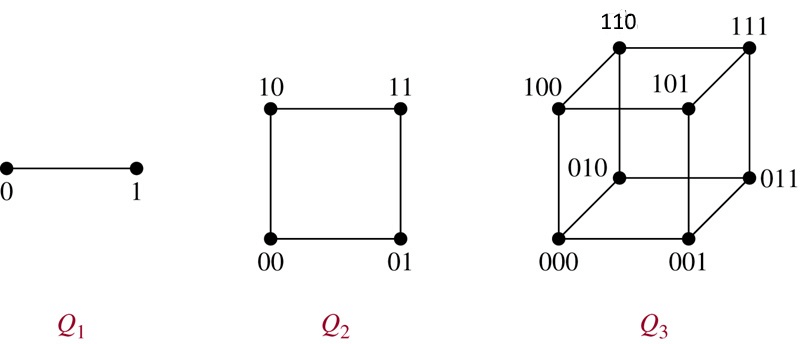
\includegraphics[width=20\linewidth]{img/Hypercube-graphs-for-n-1-2-3.png}%
    \end{minipage}}
    \item $2^n$ sommets, $deg(v) = n$
    \[ \sum_{v \in V} deg(v) = 2 |E| \implies |E| = n2^{n-1} \]
\end{enumerate}
\end{document}